\documentclass[a4papper]{article}
\title{Detecting P2P Botnets through Network Behavior Analysis and Machine Learning}
\usepackage{color}
\usepackage{ctex}
\usepackage{amssymb}
\usepackage{amsmath}
\usepackage{upgreek}
\usepackage{mathtools}
\usepackage{subfigure}
\usepackage{float}
\usepackage{indentfirst} %段落自动缩进
\usepackage{geometry}  %页边距
\usepackage{subfigure}
\usepackage{booktabs}
\usepackage{txfonts}
\usepackage{setspace}
\usepackage{natbib}
\usepackage{fancyhdr} % 添加页眉页脚
\pagestyle{fancy}%设置页眉和页脚
\lhead{}
\chead{}
\lfoot{}
\cfoot{}
\rhead{}
\rfoot{\thepage}
%\renewcommand{\headrulewidth}{0pt} %改为0pt即可去掉页眉下面的横线
%\renewcommand{\footrulewidth}{0pt} %改为0pt即可去掉页脚上面的横线 0.4pt
\usepackage[raggedleft]{titlesec} %设置标题
\usepackage{textcomp}

\renewcommand{\figurename}{Fig.}
\renewcommand{\contentsname}{目录}
\renewcommand{\thefigure}{\arabic{figure}}
\renewcommand{\tablename}{Table 1.}
\renewcommand{\thesubfigure}{(\alph{subfigure}}

\titleformat{\section}{\Huge\bfseries}{\thesection .}{.5em}{}%定义section样式
\titleformat{\subsection}{\raggedright\Large\bfseries}{\thesubsection .}{.5em}{}
\titleformat{\subsubsection}{\raggedright\large\bfseries}{\thesubsubsection .}{.5em}{}

\bibliographystyle{plain}

\geometry{left=3cm,top=3cm,bottom=4cm,right=3cm}

\author{
 Wu You\\	
 }
  \begin{document}
  	\maketitle
  	\tableofcontents
  	\thispagestyle{empty}%取消此页页眉和页脚
  \newpage
  	\setcounter{page}{1}%将此页页码计数设置为1
  	\setcounter{section}{0}%在此处将section计数设置为0,下个section将为1号
  	\section{Botnet简介}
  	\subsection{Botnet定义}
  	  	\par\setlength{\parindent}{2em} %设置段落缩进
  	Botnet也就是我们所说的Botnet网络,是指采用一种或多种传播手段,将大量主机感染bot程序(Botnet程序),从而在控制者和被感染主机之间所形成的一个可一对多控制的网络。
  	  	\par\setlength{\parindent}{2em} %设置段落缩进
  	  	往往被黑客用来发起大规模的网络攻击,如分布式拒绝服务攻击(DDoS)、海量垃圾邮件等,同时黑客控制的这些计算机所保存的信息,譬如银行帐户的密码与社会安全号码等也都可被黑客随意“取用”。因此,不论是对网络安全运行还是用户数据安全的保护来说,Botnet网络都是极具威胁的隐患。Botnet网络的威胁也因此成为目前一个国际上十分关注的问题。然而,发现一个Botnet网络是非常困难的,因为黑客通常远程、隐蔽地控制分散在网络上的“Botnet主机”,这些主机的用户往往并不知情。因此,Botnet网络是目前互联网上黑客最青睐的作案工具。
  	  	\par\setlength{\parindent}{2em} %设置段落缩进
  	  	Botnet的主要特征表现是其网络架构,根据这一特征可将其分为两类:一种是基于互联网中继聊天或HTTP协议的中心化Botnet,另一种则是基于端到端(P2P)网络结构的非中心化Botnet。其中中心化Botnet是比较容易检测和摧毁的,而端到端Botnet的检测工作则难度较大。
  	  	\par\setlength{\parindent}{2em} %设置段落缩进
  	  	有人将 Botnet攻击过程分为四个阶段,分别为:形成阶段(Formation),命令及控制(Command and Control, C and C),攻击阶段以及攻击后\cite{Leonard2009A}。多束研究工作都致力于在形成或攻击阶段对Botnet进行检测,本文主要研究在命令及控制阶段的探测问题。
  	\section{研究方法}
  	\par\setlength{\parindent}{2em} %设置段落缩进
  	对网络信息流通的分析方法分为基于端口、基于协议以及基于网络行为的分析。其中,基于端口的分析方法错误率较高,因为有大量的网络应用并不基于TCP/UDP协议来工作的。基于协议的分析方法主要通过对数据包的有效载荷(Payload)来实现,这是错误率最低的一种方法,但它同时存在两个问题,首先这种方法对计算量要求较大,会对网络性能造成影响,其次,对数据包内容的分析将涉及隐私问题。基于网络行为的分析也就是通过检测网络中的特殊行为来判断异常,由于网络日志可以从设备中轻松提取,所以这一方法对于网络性能和服务可用性的影响很小。
  	 \par\setlength{\parindent}{2em} %设置段落缩进
  	本文采用了基于网络行为的分析方法,这一方法在实际应用中所面临的问题是,Botnet的网络行为会经常发生变化,因此会产生查新问题,从而影响准确率。本文共使用了17数据特征分为基于流量和基于主机两类特征。如下图所示。\\
  	\begin{figure}[ht]
  		\centering
	  	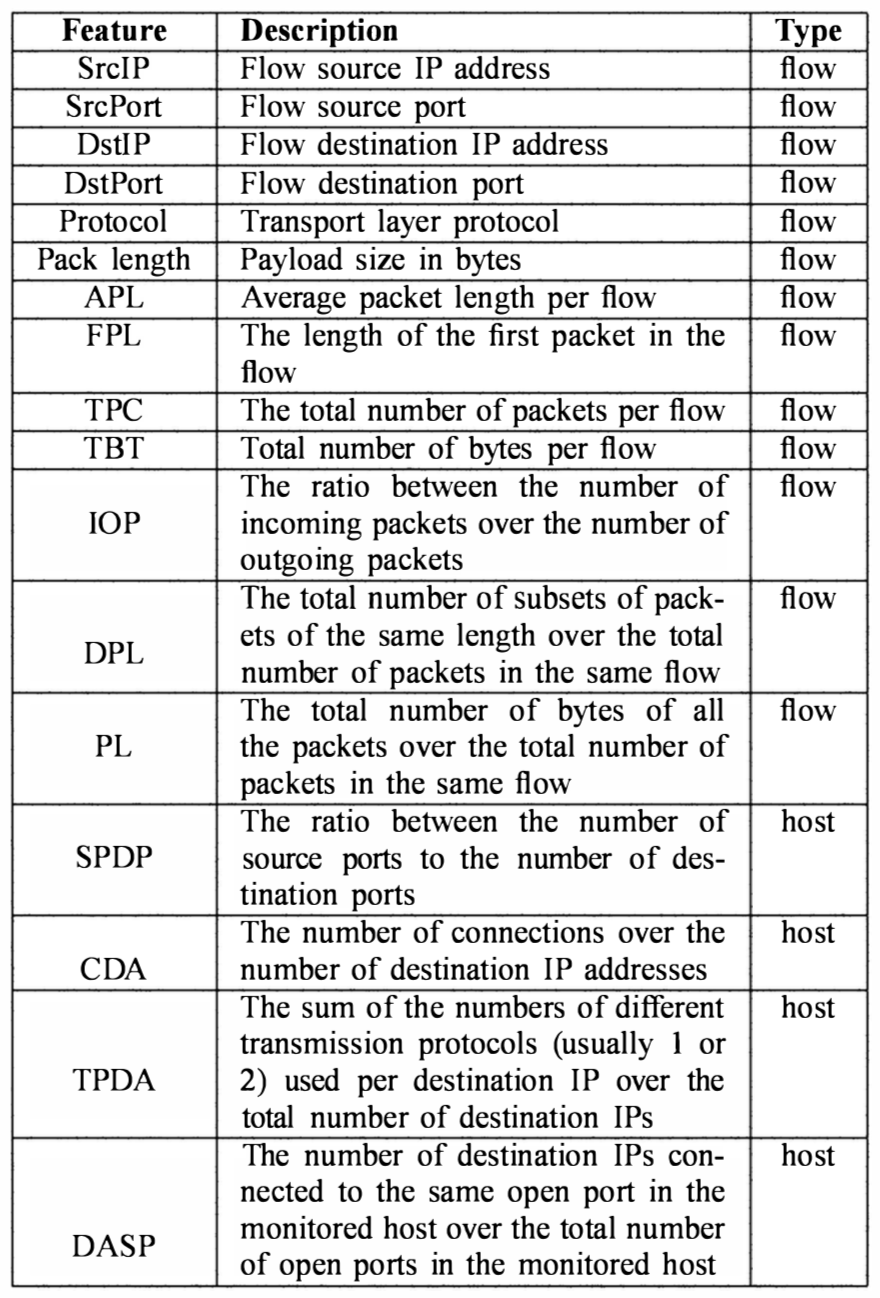
\includegraphics[scale=.5]{table1.png}  	
  	\end{figure}
  	本文选用了NNC(Nearest Neighbor Classifier),SVM,ANN,NBC以及GBC(Gaussian based classifer)算法,对其性能进行对比。
  	\section{实验结果及总结}
 	\par\setlength{\parindent}{2em} %设置段落缩进
 	以四个指标来衡量算法的性能,分别为:训练速度、分类速度、正确识别率、整体错误率。最终,NNC、ANN和SVM算法是整体性能最佳的三种算法,SVM拥有最高的正确率和最低的错误率,但训练时间和分类时间都最长。
 	存在的问题:所有的算法都无法满足查新和适应性的要求,需要一种新的算法或对算法进行混合。
  	\bibliography{battle.bib}
  \end{document}